Physical accounts complement behavioural evidence; they are not a requirement that every bodily quantity improve. A representative conservative cellular model makes that need visible: from the same acquired body and environment at step 240, continued writing and stopping new writes produce different shapes, local Food/Hazard-associated states and specific-energy fields (Fig.~\ref{fig:writing-turnover}). Continued writing retains more mass at step 560 (20.72 versus 16.13), yet more of it has low specific energy. By step 720 the mass ordering reverses (5.90 versus 8.72) while total energy has the opposite ordering (4.755 versus 1.170). Reduced injury loss is outweighed by additional starvation loss. This no-birth model retains decay, eligibility and transport after writing stops. Its local fields are observations of coupled dynamics, not isolated mediators or tracks of the same material.



Two other comparisons identify what must be controlled when an experienced body survives better. Continued actor updating can preserve mass and energy mainly by reducing motor payment, with little additional intake; retained-state expression can likewise save energy while uptake remains small (Supplementary Figs.~\ref{fig:action-renewal} and \ref{fig:action-opportunity}). These findings motivate reachable, replenished opportunities and separate ledgers for intake and action costs in the new task. They do not establish that a surviving actor acquired a better model of its environment. Matching initial action probabilities is also insufficient to match realized actions, contacts and expenditure.

\begin{figure}[p]
\centering
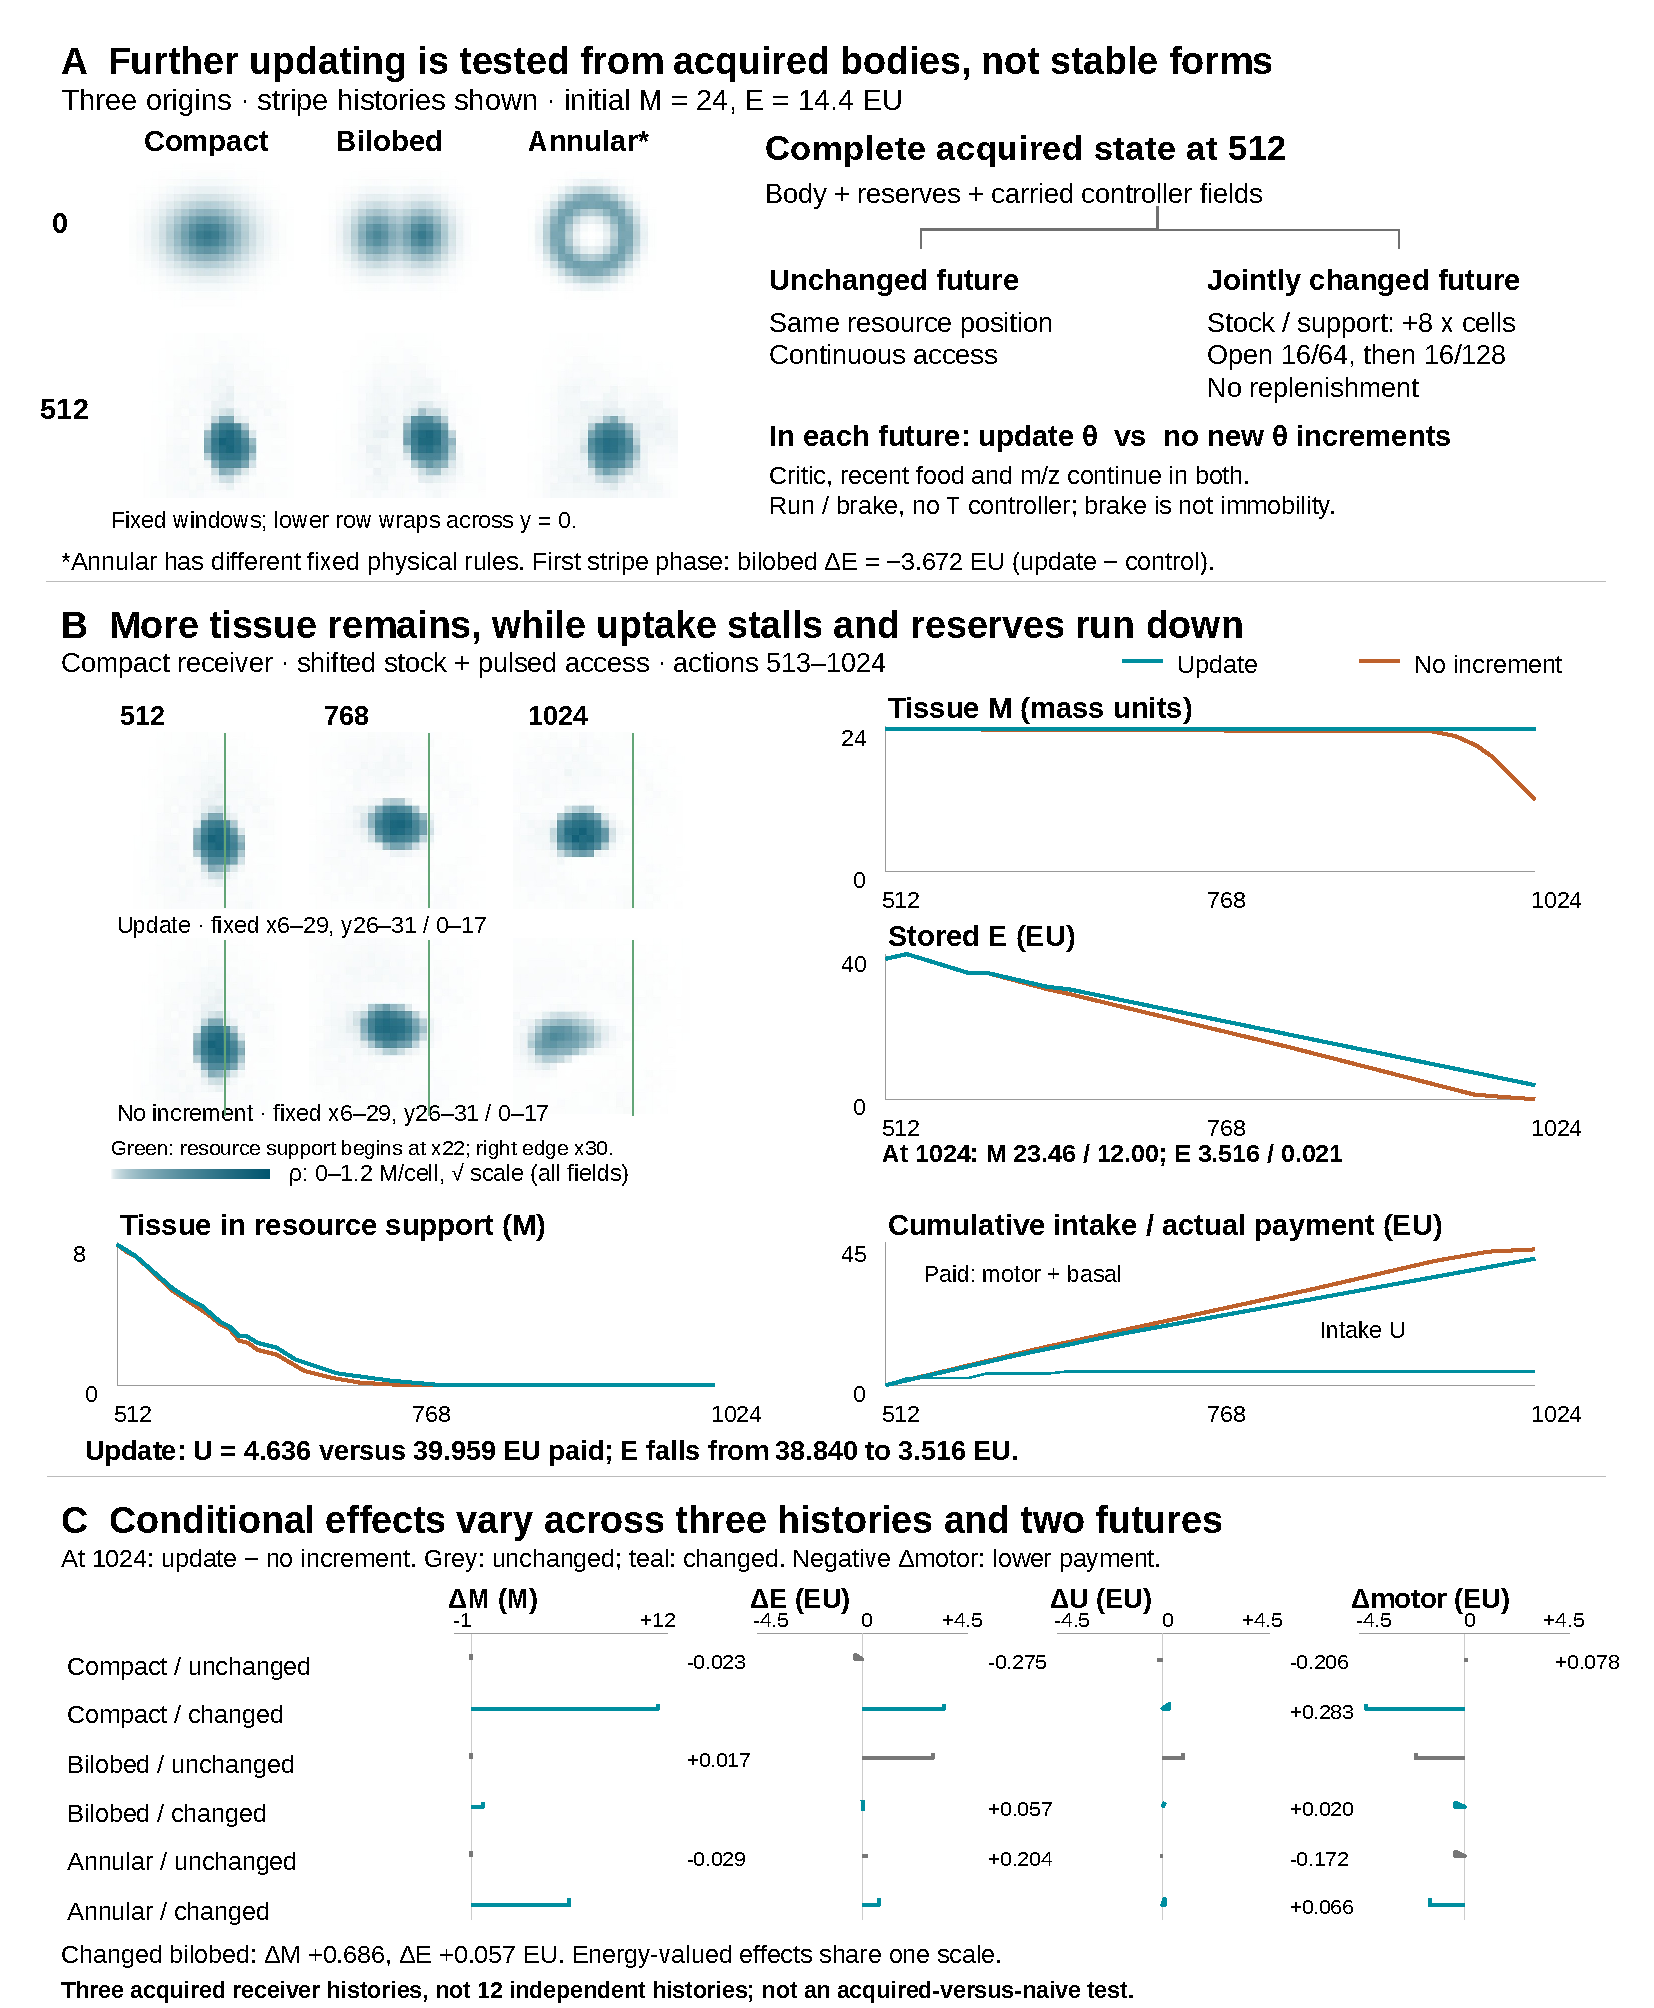
\includegraphics[width=0.90\linewidth]{figures/main/action_updating/adaptive_action_renewal.pdf}
\caption{\textbf{Continued action updating can retain tissue without sustaining substantial acquisition.}
\textbf{a,} Three structural origins and their acquired stripe states at step 512, shown in fixed original-coordinate windows; the lower window crosses the periodic $y$ boundary. Names denote origins, and the annular origin uses different fixed physical coefficients. Each acquired complete state supplies unchanged and jointly shifted/pulsed futures, each with or without further actor-logit increments. Other online processes continue; the run/brake controller has no interval $T$, and braking suppresses polarity readout rather than immobilizing tissue.
\textbf{b,} Compact origin under the changed future. Original-coordinate density windows, resource-support tissue and whole-body stock/receipt curves show that the larger retained mass coexists with very low late uptake and declining reserves. Green lines mark the resource support, not whether access is currently open. Actual payments combine motor and basal costs; energy lost with tissue is separate. Curves use archived per-action ledgers, rendered as simplified native polylines.
\textbf{c,} All six continuation contrasts (update minus no further increments). Energy-valued contrasts share one scale. The three acquired histories are not twelve independent histories. These conditional continuation effects do not measure acquired-versus-naive transfer benefit or establish sustained adaptation.}
\label{fig:action-renewal}
\end{figure}

\begin{figure}[p]
\centering
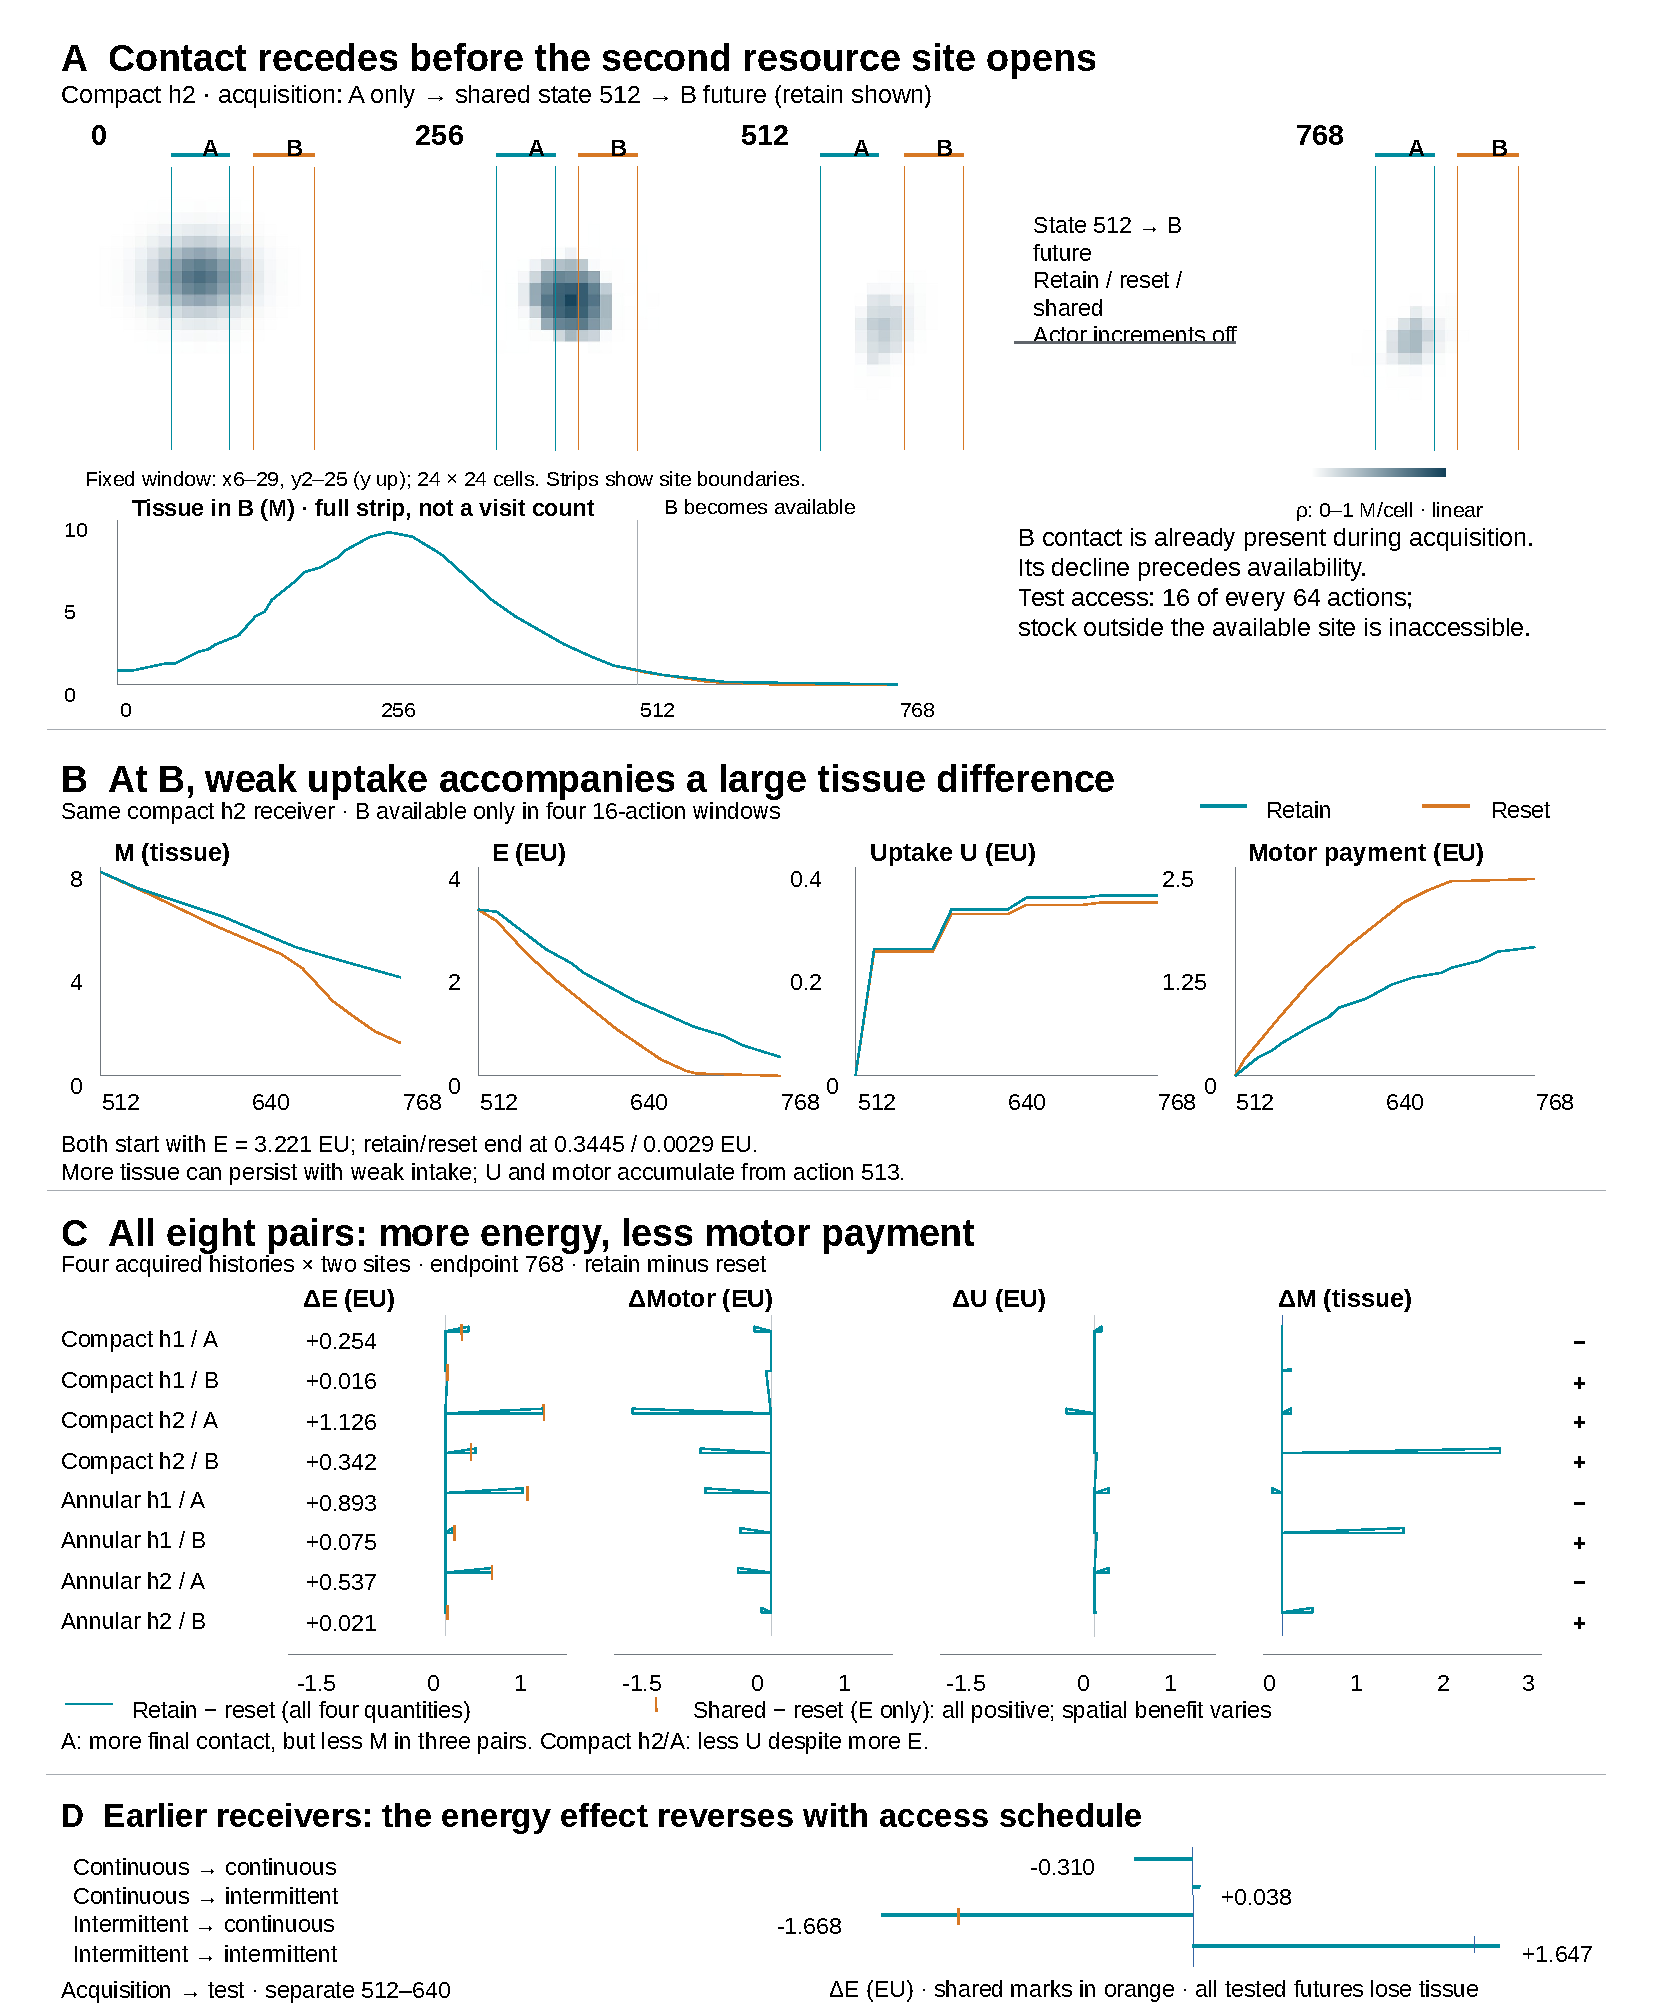
\includegraphics[width=0.94\linewidth]{figures/main/action_opportunity/action_opportunity.pdf}
\caption{\textbf{Retained actor state can preserve energy without restoring substantial uptake.}
\textbf{a,} Compact h2 body fields in one original-coordinate window (x6--29, y2--25; y upward), with common linear density scale. Lines locate resource strips, not stocks. Only A supplies during acquisition; B becomes available at 513. Full-strip B contact rises and then recedes before availability.
\textbf{b,} Absolute tissue, energy and cumulative uptake/motor payment from the same receiver at 512. Retaining more tissue accompanies weak uptake and reserve depletion.
\textbf{c,} All eight conditions from four histories and two future sites. Teal: retain minus reset; orange: shared minus reset for energy. The three EU quantities share a scale; tissue has its own scale. Higher A contact does not ensure more total tissue or uptake.
\textbf{d,} A separate earlier batch crosses two compact acquisition histories with two test schedules (512--640), giving opposite energy signs under continuous and intermittent access; orange marks add the one-receiver shared diagnostic. Actor increments are disabled throughout these tests. Initial mean probability matching does not match actions or payments. These conditional retained-state effects do not establish sustained adaptation.}
\label{fig:action-opportunity}
\end{figure}


The bodily return itself has non-interchangeable components. In producing bodies, independently enabling precursor P transport increases final mass and integrated body-time but reduces final energy; fuel F transport improves energy throughout the tested window while its mass effect depends on body and time (Fig.~\ref{fig:allocation-feedback}). At the first matched action, P transport exposes an existing F restriction: sequential F rejection increases although the actual F field and independently evaluated deficit are unchanged. Later organization diverges, so that comparison does not establish a fixed-organism mediator for the whole path. Porous branches lose late mass while four-lobed branches grow; short negative interaction intervals and real micro-starvation losses remain in the full accounts. These comparisons justify testing useful decisions against multiple physical outcomes, rather than treating tissue gain, stored energy or rejection counts as interchangeable rewards.



Finally, a useful learned state must be distinguished from the body's inherited capacity and the persistence of its carrier. Generative rules can produce growing forms without establishing stable maintenance (Supplementary Fig.~\ref{fig:formation-persistence}). An offspring can inherit finite-window injury tolerance while its own experience still lowers energy and complete body-time; a different lineage loses performance under its own rule replacement (Supplementary Fig.~\ref{fig:inheritance-recovery}). These package interventions are not pure shape changes or the same numerical mutation across lineages. Paid copying can preserve a protection state after the original tissue cohort disappears, yet late erasure need not remove finite persistence (Fig.~\ref{fig:paid-protection-renewal}). Together these results define the required distinction between acquired information, developmental carryover and material replacement. Their detailed trajectories remain supporting mechanistic comparisons; they are not additional demonstrations of the candidate learning rule.

\begin{figure}[p]\centering
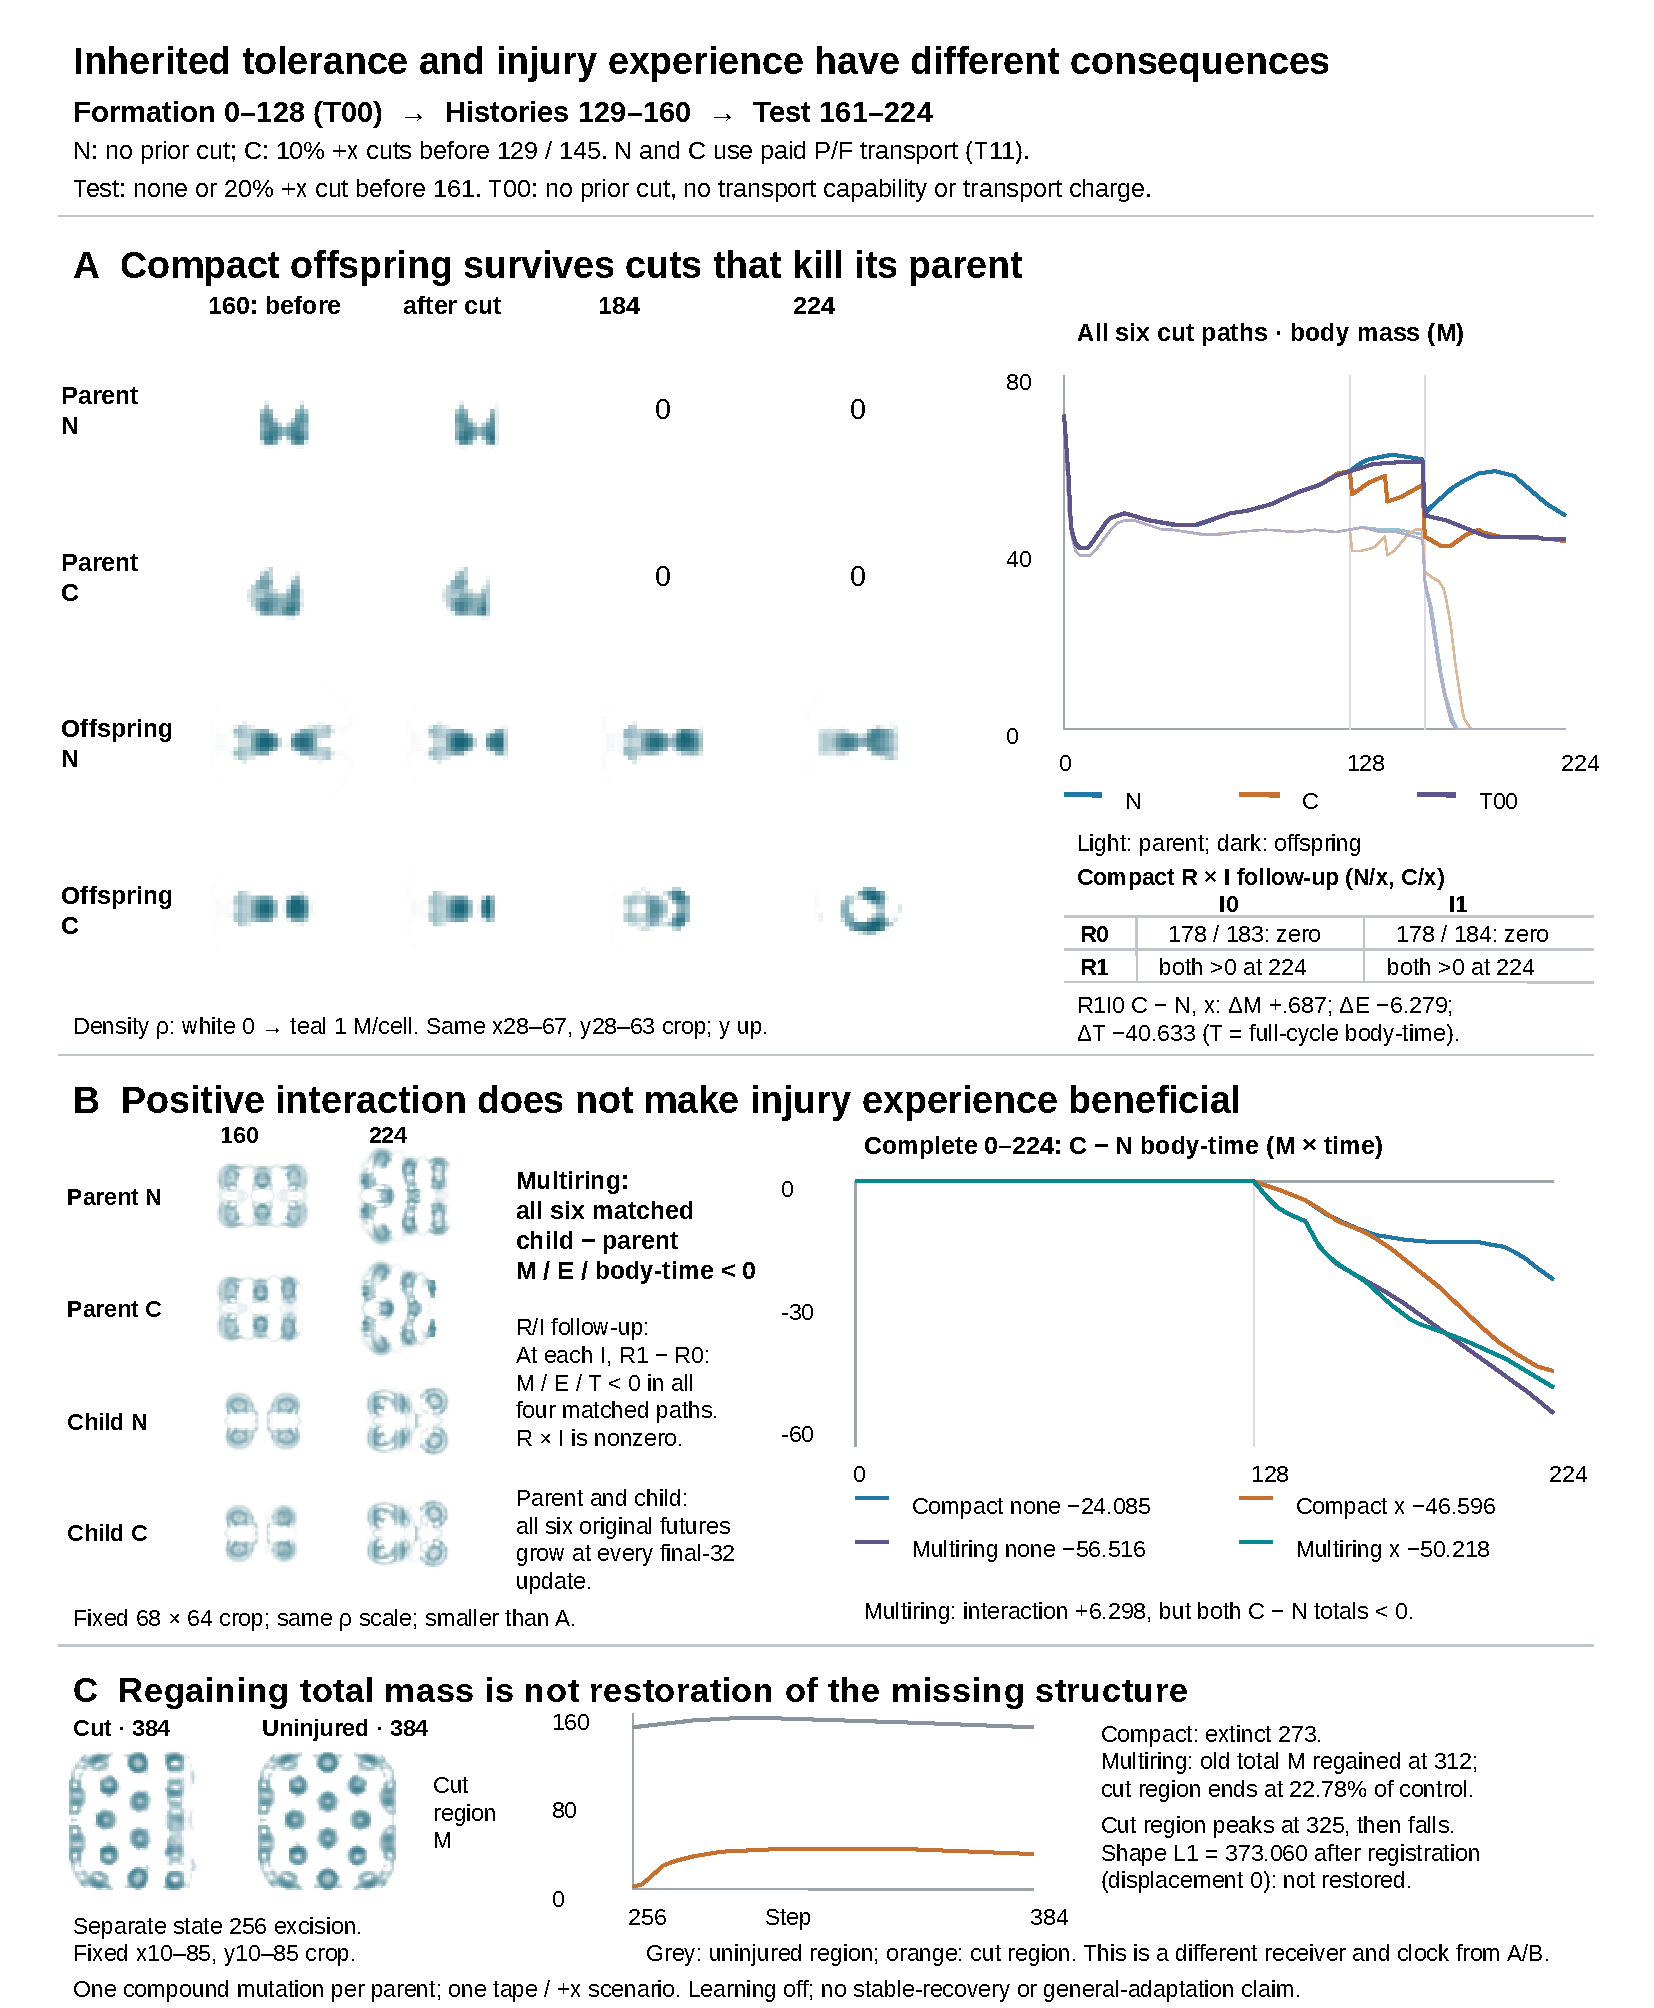
\includegraphics[width=\linewidth,height=.77\textheight,keepaspectratio]{figures/main/inheritance_recovery/regenerative_inheritance_recovery_factorial.pdf}
\caption{\textbf{Inherited tolerance, injury experience and local restoration are distinct.} \textbf{A,} Compact parent/offspring fields and complete challenged paths preserve parental extinction and zero tails. A separate rule--initial matrix shows survival through 224 under both offspring-rule combinations; experienced-minus-naive energy and body-time can nevertheless fall. R contains both kernels and complete response parameters; I contains density, energy, founder and polarity fields. \textbf{B,} The multiring offspring loses in all six matched paths, and the rule cross remains adverse under both I. Both offspring's complete experienced-minus-naive body-time paths are negative. \textbf{C,} An independent state-256 excision receiver regains total mass while its fixed original cut region remains depleted and later shrinks. Original coordinates, terminal uninjured reference and local trajectories distinguish total growth from restoration. Panels have distinct clocks and dependent paths; no learning or general recovery is established.}
\label{fig:inheritance-recovery}\end{figure}


\begin{figure}[p]\centering
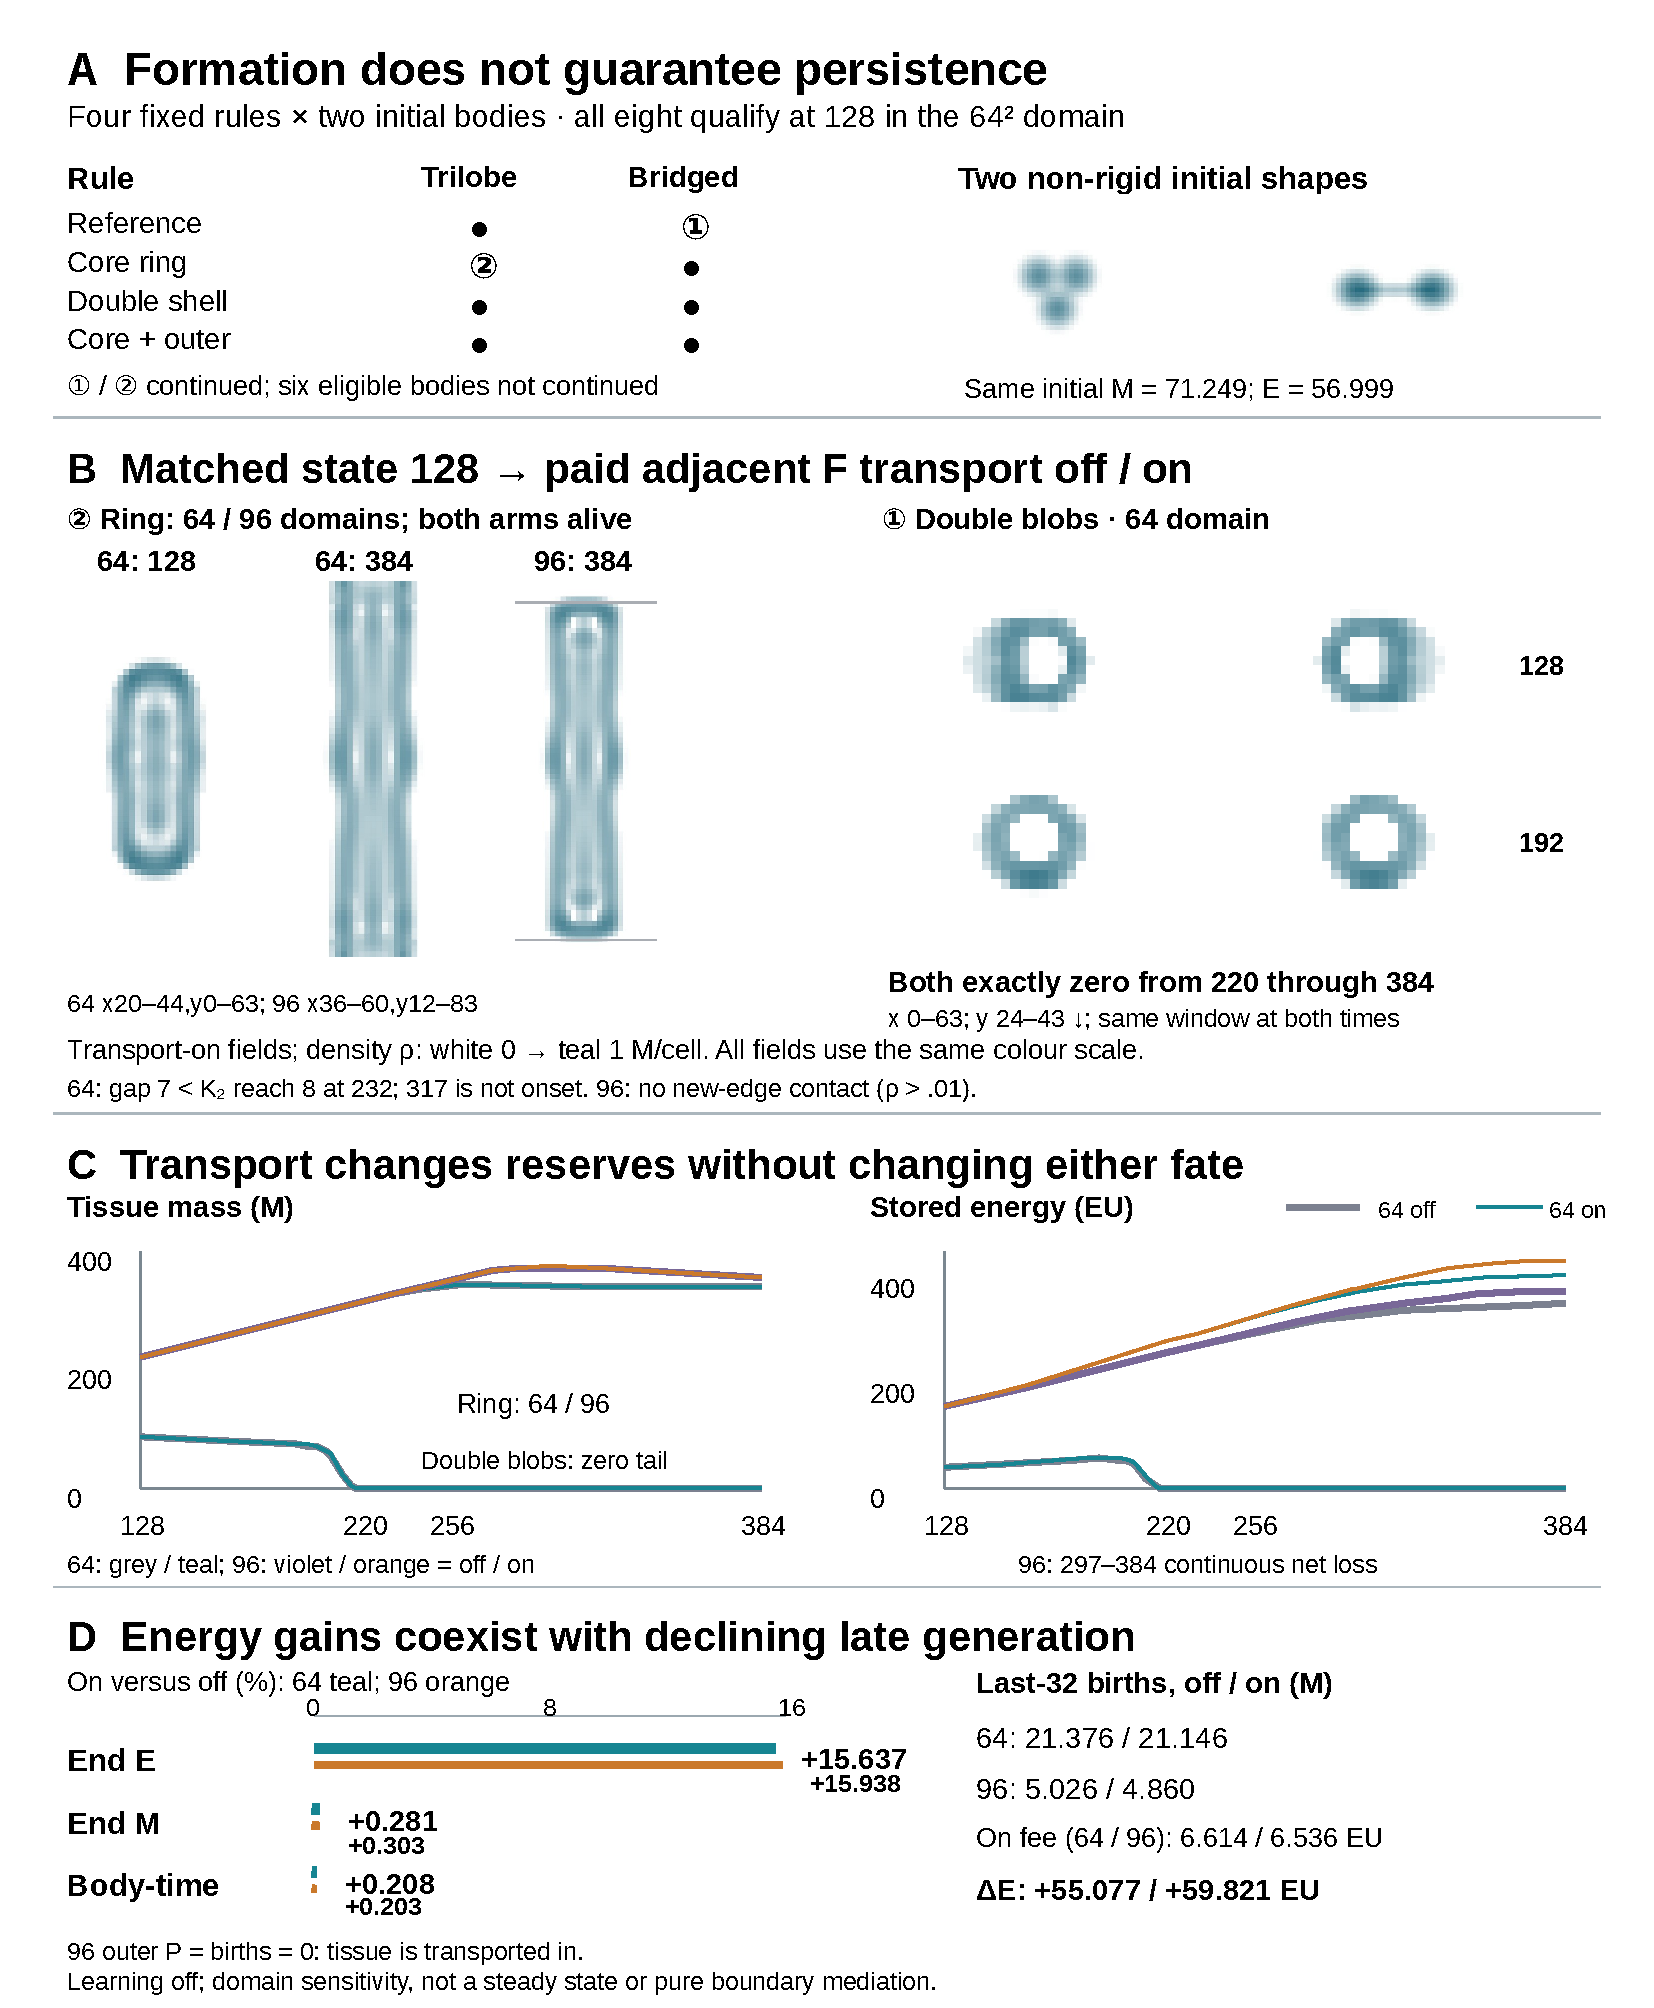
\includegraphics[width=\linewidth,height=.76\textheight,keepaspectratio]{figures/main/formation/regenerative_morphology_transport.pdf}
\caption{\textbf{Formation, persistence and the energetic value of fuel transport differ.} \textbf{a,} Eight rule/initial-field combinations qualify at 128; six are uncontinued. \textbf{b,} True density fields preserve original coordinates and a common scale. Both separated-body futures become extinct; the ring persists in both domains. \textbf{c,} Complete mass and energy paths retain zero tails and late loss. \textbf{d,} Within-domain on-minus-off effects show much larger energy than tissue/body-time gains. Outer tissue in the larger domain arrives by transport without local birth in this comparison. The embedding changes the whole domain condition, not an isolated boundary mediator. These selected dependent paths do not establish learning or stable maintenance.}
\label{fig:formation-persistence}\end{figure}





\begin{figure}[p]
\centering
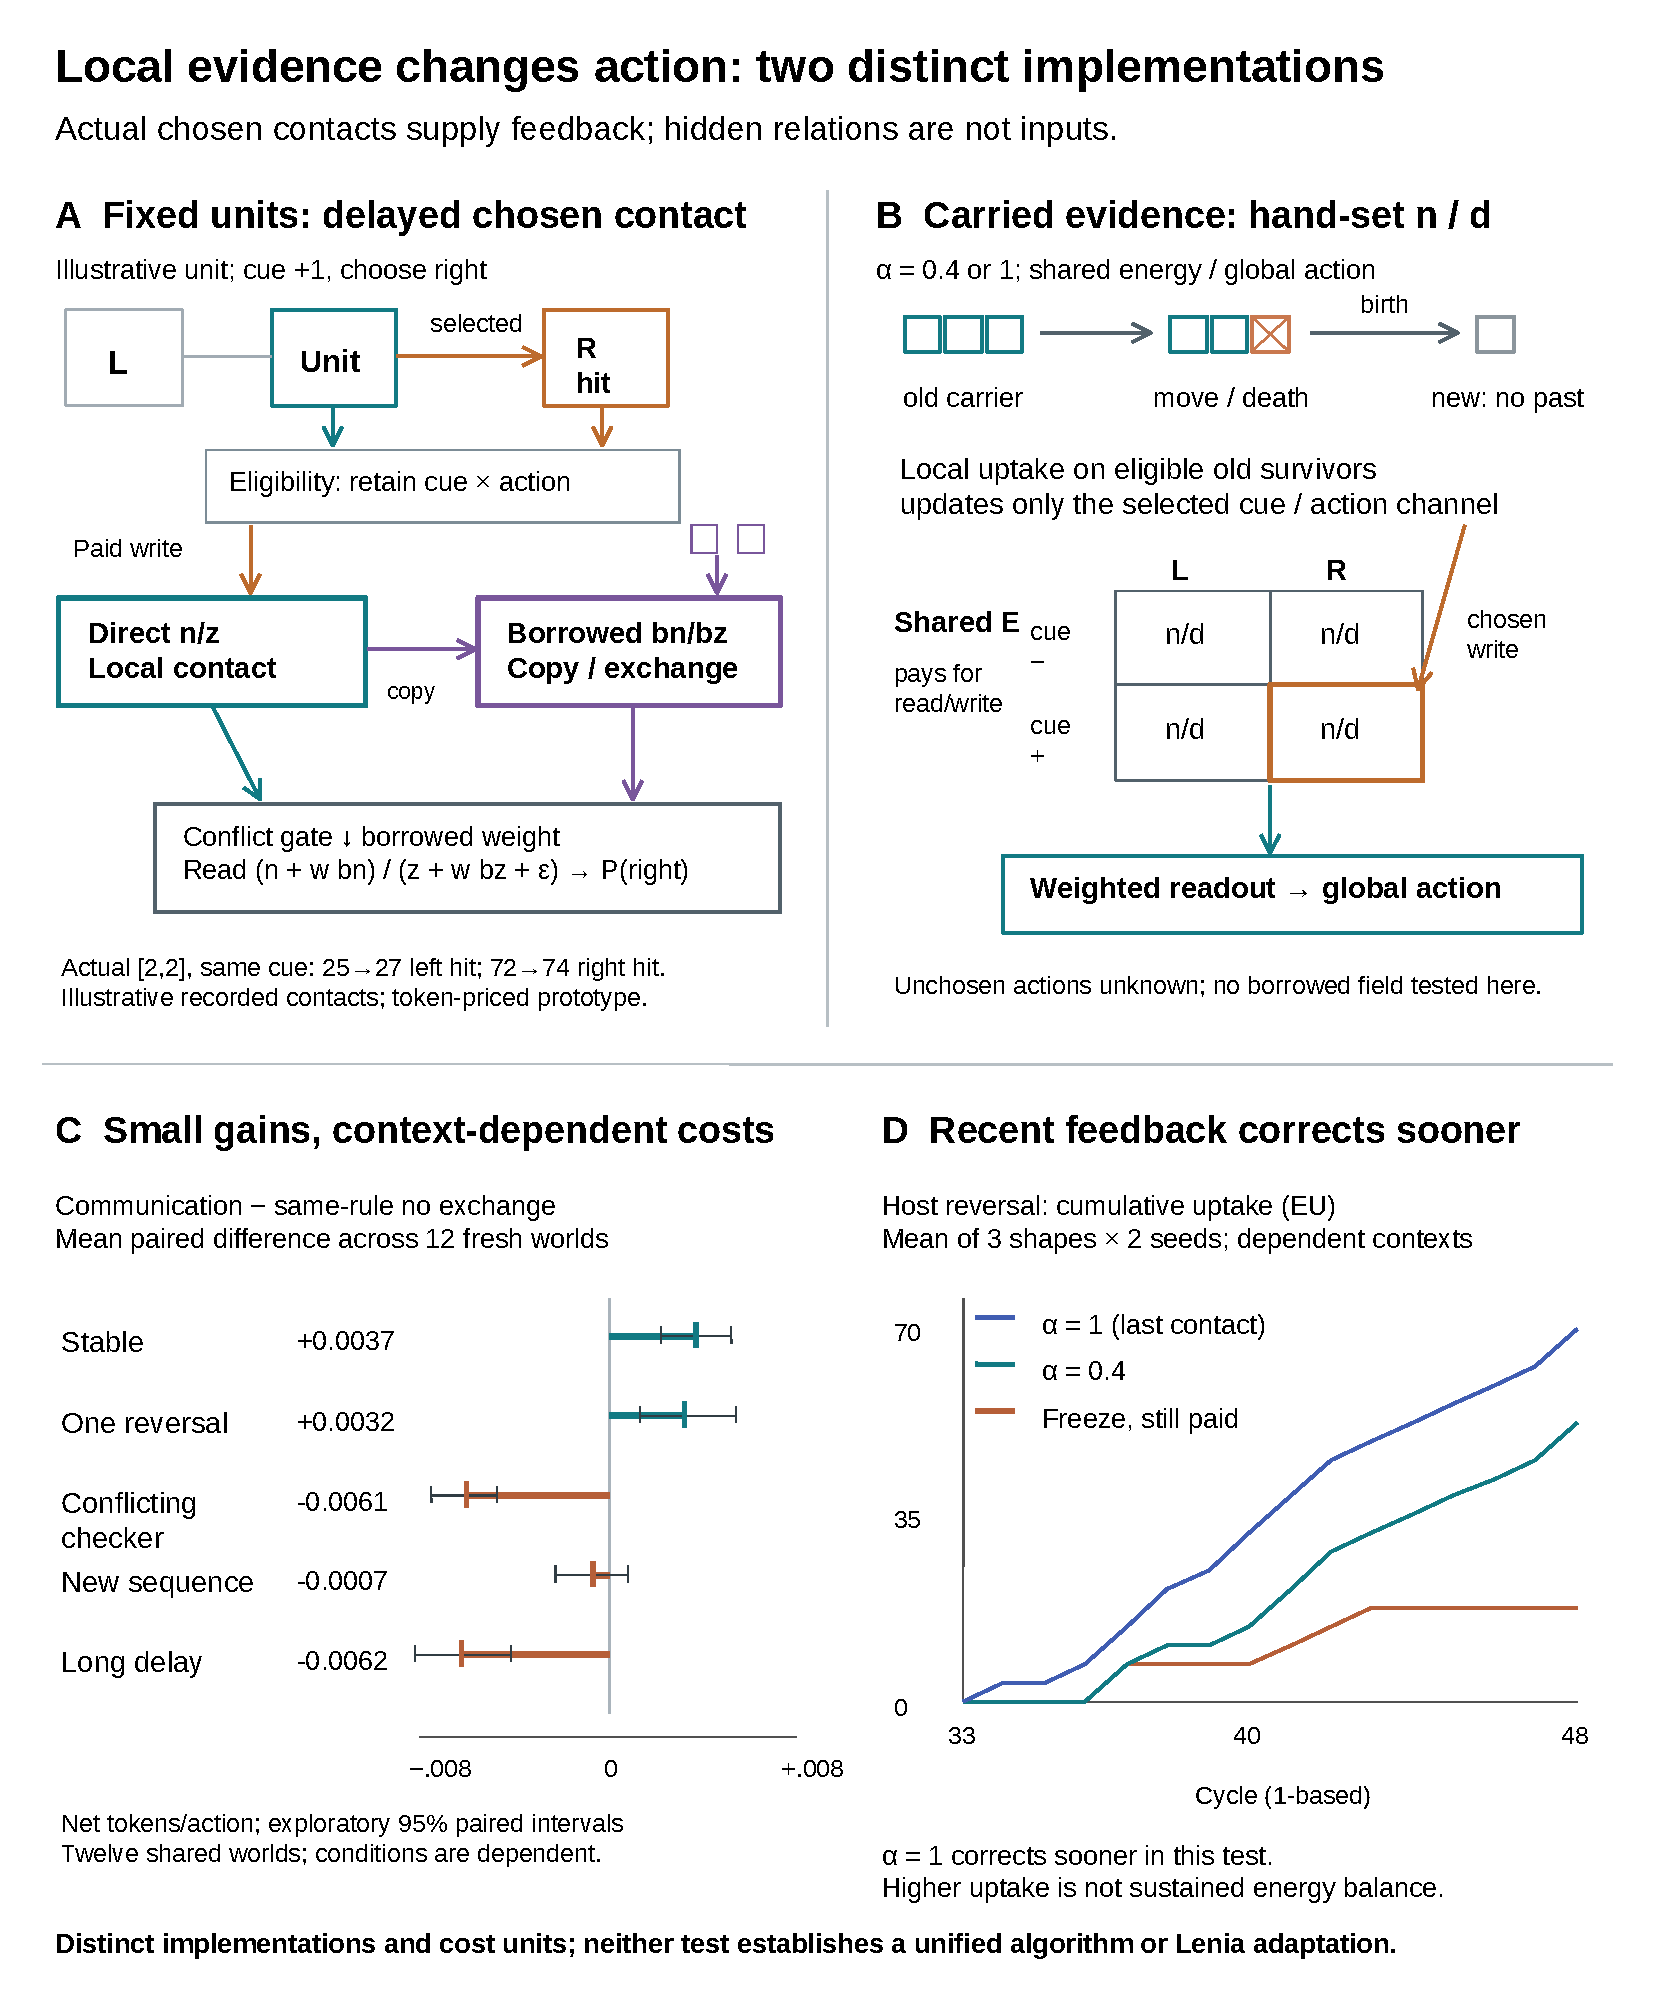
\includegraphics[width=\linewidth,height=0.79\textheight,keepaspectratio]{work/method_renewal/figures/local_evidence/local_evidence.pdf}
\captionsetup{font=footnotesize}
\caption{\textbf{Delayed local evidence connects encounters to later choices in two distinct implementations.}
\textbf{a}, Fixed contact units retain cue--action eligibility until an actual contact returns. Paid writes update direct evidence; a separate channel carries received estimates, whose influence is reduced by conflict with confident direct evidence. These units have token costs but no changing body.
\textbf{b}, A separate hand-set estimator attaches cue eligibility and uptake evidence to a moving density host. Surviving old carrier can write from local uptake; transport and death carry or remove stored state, while newborn tissue starts without past experience. A global readout and common energy reserve control movement and payment. This host does not implement the separated-message rule in \textbf{a}.
\textbf{c}, Communication minus no exchange at identical rule parameters: mean net-token differences across twelve paired world seeds. Intervals are exploratory 95\% paired bootstrap intervals. The same worlds recur across conditions.
\textbf{d}, Cumulative actual uptake after a new host reversal, averaged over three prescribed shapes sharing two environmental seeds. The latest-contact rate $\alpha=1$ corrects sooner than $\alpha=0.4$; paid freezing stops value writes. Increased uptake does not establish energy balance.}
\label{fig:local-evidence}
\end{figure}

